\documentclass{article}
\usepackage[utf8]{inputenc}
\usepackage[spanish]{babel}
\usepackage{graphicx}
\graphicspath{ {images/} }



\begin{document}

\begin{titlepage}
    \begin{center}
        \vspace*{1cm}
        
        \Huge
        \textbf{Informe Parcial 1}
            
        \vspace{0.5cm}
        \LARGE
       \textit{ Informática II}
            
        \vspace{1.5cm}
            
        \textbf{Juan Sebastian Garavito Gallo\\
        Anderson Giraldo Arboleda\\
        Jesus David Mercado Machado}
            
        \vfill
            
        \vspace{0.8cm}
            
        \Large
        Despartamento de Ingeniería Electrónica y Telecomunicaciones\\
        Universidad de Antioquia\\
        Medellín\\
        2022
            
    \end{center}
\end{titlepage}

\tableofcontents
\newpage

\section{RESUMEN}
\label{resumen}




\newpage
\section{INTRODUCCIÓN}

\newpage
\section{TAREAS}
\label{tareas}
Definimos las tareas para el desarrollo de la solucion del problema de la siguiente manera.

\begin{itemize}

    \item La primera tarea que tuvimos que resolver fue entender el problema y hacerle su debido análisis.
    
    \item Despues del análisis, empezamos a investigar sobre el dispositio y amontar los jemplos en tinkercad que nos ayudaran a comprender el funcionamiento del mismo.
    
    \item Luego de tener la bandera empezaremos con el desarrollo del algoritmo.
    
    \item 
    
   
    
\end{itemize}


\newpage
\section{ANÁLISIS DEL PROBLEMA}
\label{Análisis}

El sistema básicamente se dividirá en tres partes, el Arduino emisor que mediante su puerto serial recibirá la cadena de números enteros y enviara los datos al Arduino receptor, mientras que paralelamente con la ayuda de un circuito adjunto se comprobara byte a byte si el número ingresado es la bandera entregada o no. Por último el Arduino receptor, recibe tanto los datos enviados que ira guardando en un arreglo dinámico como la comprobación de la bandera, que indicara el comienzo del proceso de descripción en el Arduino receptor, de proceso saldrá el mensaje verdadero que posteriormente se mostrara mediante el puerto serial en el pc2.


\newpage
\section{MARCO TEÓRICO}
\label{marco}
\item 1. [20] Investigar y explicar con sus propias palabras cómo utilizar el circuito integrado 74HC595. En esta parte mostrar un ejemplo de uso del circuito integrado primero de forma independiente con pulsadores o switches y luego usando Arduino,y detallar en el informe la utilidad que puede darle a este elemento para la solución del problema.\\

-Es un registro de desplazamiento que cuenta con una entrada en serie y salida en paralelo de 8 bits. Este dispositivo solo funciona con dos valores de tensión 1 y 0, 1 sería el valor +Vcc y 0 un valor muy cercano a 0v.\\

-Se puede tomar como un conversor de serie-paralelo. Como es de suponer la entrada se dará un valor uno detrás de otro, mientras que su salida mostrará todos los entregará a la vez.\\

-Otro factor importante de este componente es que cada vez que se le entreguen datos nuevos el no los va a sobrescribir lo que hará es desplazarlos n posiciones a la derecha, siendo n el número de datos nuevos.\\

-Una de las utilidades que nos puede entregar este elemento para la solución del problema es el clock de latch lo que quiere decir que hasta que no llegue un flanco de subida por el clock de latch los shift registrer no pasan a la salida permitiendo esto organizar los datos con completa libertad sin ir a afectar el circuito.\\

-Para el caso es muy útil ya que si no existiera el latch veríamos todo el proceso de encriptación mientras se organiza, viendo así datos o valores que no son lo que realmente queremos, mientras que con esto podemos ordenar los datos y cuando realmente deseemos mostrarlo.\\

-Otra gran ventaja que es muy útil de este componente es reducir el número de pines que se necesitaría para llevar a cabo una tarea, lo reduce a 3 pines. Si por ejemplo tenemos varios componentes iguales y conectamos la salida del shift a con la señal de siguiente “conectarlos en cascada” podemos incrementar el número de elementos a controlar sin que suba el nuero de pines.\\
\\
\\
\\
\\
\\
\\
\\
\\
\\
Ejemplo para el componente con pulsadores y sin Arduino\\

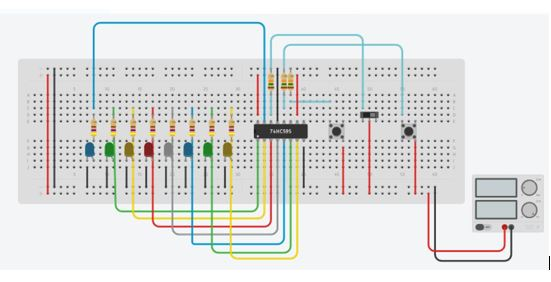
\includegraphics{Captura1.JPG}





\newpage
\section{EVOLUCIÓN DEL ALGORITMO}
\label{evolucion}



\end{document}
